%Revisando

Este capítulo detalha os procedimentos metodológicos e as ferramentas desenvolvidas para a aquisição e o processamento de dados, que constituem a base para o treinamento e a validação do sistema de visão computacional proposto. O \textit{pipeline} sistemático desenvolvido nesta pesquisa é estruturado em quatro etapas consecutivas, integrando os universos de engenharia de \textit{hardware} e \textit{software}: (i) \textbf{Aquisição física}: captura estandardizada das amostras de algodão em pluma utilizando a cabine fotométrica autoral sob dupla temperatura de cor; (ii) \textbf{Pré-processamento visual}: segmentação semântica robusta de fundo via BiRefNet e eliminação cromática no espaço HSV; (iii) \textbf{Engenharia de dados (recorte em blocos)}: extração geométrica da Região de Interesse (ROI) via algoritmo do Maior Retângulo Interno (LIR) e fragmentação estratificada em blocos de $256 \times 256$ pixels; e (iv) \textbf{Modelagem profunda}: processamento, treinamento bayesiano e classificação preditiva por meio das 17 arquiteturas neurais de estado da arte avaliadas. Estas quatro etapas conceituais desdobram-se nas sete seções deste capítulo: as Seções \ref{sec:sistema_aquisicao} e \ref{sec:protocolo_coleta} detalham a aquisição física; a Seção \ref{sec:prepdados} cobre o pré-processamento visual e a engenharia de dados; a Seção \ref{sec:conjunto_dados} descreve a construção do conjunto de dados; e as Seções \ref{sec:modelos}, \ref{sec:ambiente_treinamento} e \ref{sec:desenho_experimental} detalham a modelagem profunda e o desenho experimental. Cada etapa foi projetada com foco na robustez da luminosidade, na padronização das amostras e na reprodutibilidade dos resultados.


\section{Desenvolvimento do Equipamento de Coleta de Imagens}
\label{sec:sistema_aquisicao}

    %Revisado

A estrutura física consiste em uma cabine retangular fechada, construída em MDF, com dimensões de $40 \times 40 \times 60$ cm (largura, profundidade e altura). O materia, de cor branca e opaca, possui o duplo objetivo de bloquear a luz externa e evitar a contaminação colorimétrica por reflexos das paredes. O equipamento possui um compartimento superior isolado para acomodar as fontes de alimentação e a eletrônica, garantindo que a área inferior de captura fique livre de cabos e sombras indesejadas. O dispositivo de captura foi montado centralizado no teto da estrutura, a uma distância focal aproximada de 40 cm da base onde as amostras são introduzidas (através de uma abertura frontal), garantindo um enquadramento constante. Um esquema técnico detalhado do equipamento é apresentado na Figura \ref{fig:caixa}.

O sistema de iluminação foi projetado estrategicamente para lidar com os desafios ópticos da pluma de algodão. Utilizaram-se duas matrizes de fitas de LED de alta intensidade (2000 lm/m) posicionadas na parte superior, fornecendo luz difusa para minimizar a geração de sombras profundas e brilhos especulares na fibra. O sistema permite a alternância de temperaturas de cor: LEDs de 2800K (luz ``quente'') foram empregados para realçar a reflectância e o amarelamento natural da fibra (+b), enquanto LEDs de 6000K (luz ``fria'', próxima à luz do dia) maximizaram o contraste morfólogico das impurezas superficiais. O protocolo de captura gerou três imagens por amostra: apenas 2800K, apenas 6000K, e ambas simultaneamente, compondo um \textit{dataset} multiespectral robusto para o treinamento das redes.

O módulo de aquisição baseou-se em um sensor CMOS operando a uma resolução de $1280 \times 720$ \textit{pixels}. Optou-se por esta tecnologia devido à sua alta viabilidade de implantação em esteiras industriais, unindo baixo custo e baixo consumo energético, conforme fundamentado na revisão de literatura. O sensor foi acoplado a uma lente grande-angular com campo de visão de 140°, o que permitiu maximizar a área de amostragem do algodão capturada na base do equipamento sem a necessidade de elevar a altura da caixa. As distorções geométricas inerentes a lentes de grande angulação foram mitigadas pelo posicionamento centralizado da amostra.


\begin{figure}[H]
\centering
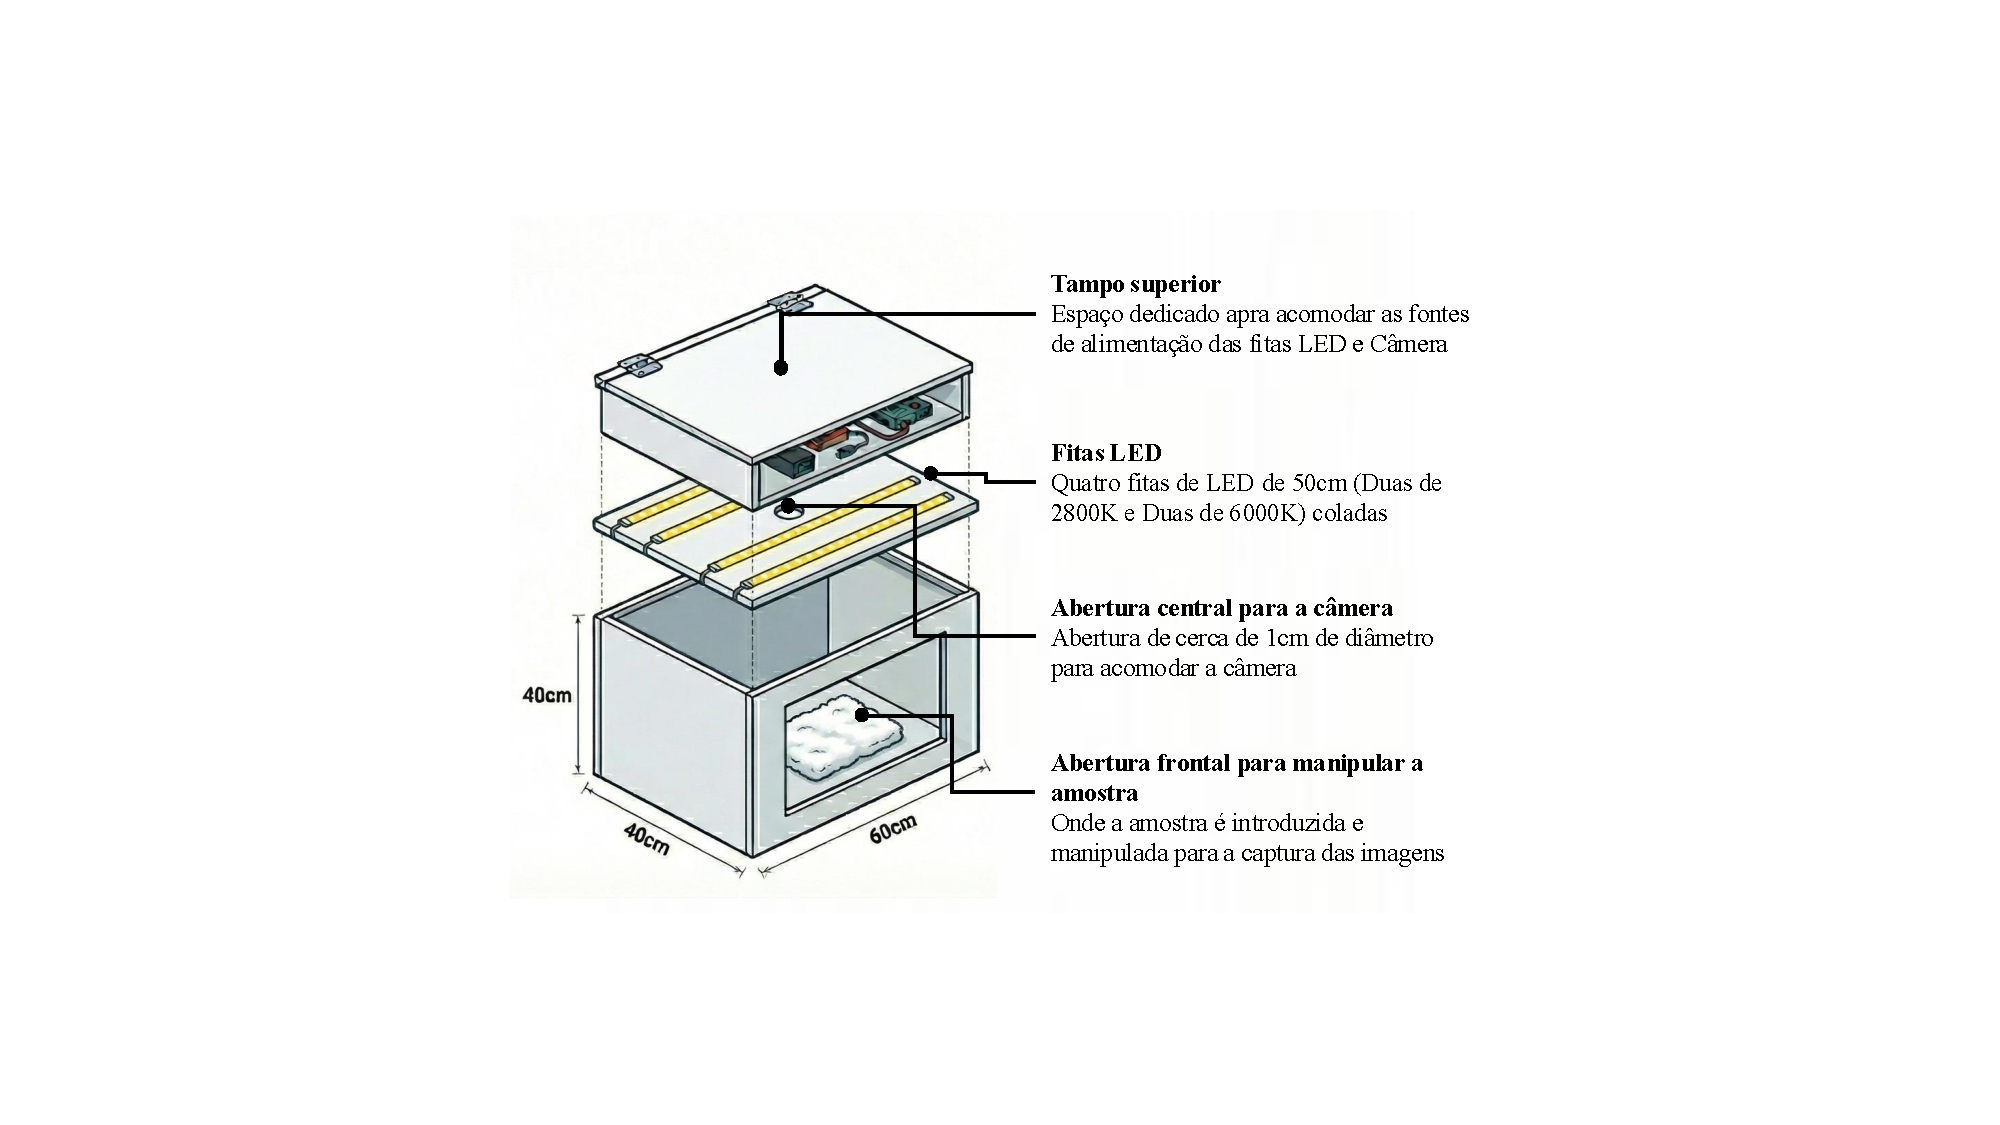
\includegraphics[trim=7.5cm 4cm 7.5cm 4cm, clip, scale=0.9]{images/img_caixa_3.pdf}
% \vspace{-1cm}
\caption{Equipamento de coleta de amostras}
\label{fig:caixa}
\end{figure}

\section{Protocolo de Coleta e Amostragem}
\label{sec:protocolo_coleta}

    %Revisado

O processo de aquisição de dados foi conduzido em ambiente industrial, diretamente nas instalações de uma unidade de beneficiamento de algodão (algodoeira) localizada no município de Sapezal, Mato Grosso, um dos principais polos produtivos do cerrado brasileiro. A coleta ocorreu durante o beneficiamento safra de 2023/2024, totalizando 3.852 imagens brutas, sendo 1.284 para cada uma das três configurações de iluminação (2800K, 6000K e ambas).
    
Para garantir a rastreabilidade e a reprodutibilidade do experimento, estabeleceu-se um protocolo padronizado de captura, desenhado não apenas para gerar as imagens, mas para assegurar o vínculo exato com os laudos de qualidade oficiais (o \textit{ground truth} dos modelos). O fluxo de trabalho operacionalizou-se nas seguintes etapas, ilustradas no fluxograma da Figura \ref{fig:fluxograma_coleta}\footnote{Um vídeo demonstrativo da operação do sistema de captura na unidade de beneficiamento pode ser acessado no Material Suplementar ou por meio do link: \url{https://www.youtube.com/shorts/d_1C78sa11c}}:

\begin{enumerate}
    \item \textbf{Identificação e Rastreabilidade:} O operador inicia o ciclo utilizando um leitor de código de barras para escanear a etiqueta universal da amostra. Ess procedimento vincula automaticamente o ID único do fardo, o lote de processamento e a origem da pluma aos metadados dos arquivos de imagem que serão gerados, eliminando o risco de erros de digitação e garantindo o cruzamento futuro com os dados de classificação oficial (HVI/Visual).
    
    \item \textbf{Posicionamento Padronizado:} A porção de algodão é extraída de sua embalagem e alocada no centro da base do equipamento de captura. O operador realiza a padronização manual do formato da amostra, acomodando a superfície da pluma para garantir a máxima planicidade possível. Esse rigor na modelagem física da amostra é crucial para evitar oclusões severas, minimizar a formação de sombras irregulares e assegurar que a área exposta à lente seja representativa da densidade real do fardo.
    
    \item \textbf{Captura Multiespectral:} Por meio da interface do \textit{software} de controle, a sequência de aquisição é disparada. O operador orquestra manualmente o acionamento dos LEDs e a captura das imagens em três condições sequenciais: iluminação exclusiva de 2800K (AM), iluminação exclusiva de 6000K (BR) e iluminação combinada (AB). As três matrizes de pixels resultantes são armazenadas em um diretório em formato sem perdas (PNG) e atreladas ao ID escaneado no Passo 1.

    \item \textbf{Encaminhamento para Classificação Oficial:} Concluída a aquisição visual, a amostra física é imediatamente reconduzida ao fluxo normal da algodoeira, sendo destinada ao laboratório para a classificação comercial humana. Esse passo é o que permite a rotulagem supervisionada do conjunto de dados nas etapas posteriores da pesquisa.
\end{enumerate}


\begin{figure}[ht!]
\centering
\caption{Fluxograma do processo de coleta de amostras e aquisição de imagens.}
% --- Definição dos estilos dos elementos do fluxograma ---
%   \tikzset{
%     process/.style    = {rectangle, rounded corners, draw, fill=blue!10, text width=7.5em, text centered, minimum height=2em, node distance=1.5cm},
%     startstop/.style  = {circle, draw, fill=green!20, text centered, minimum height=2em, node distance=0.5cm},
%     arrow/.style      = {-{Stealth[]}, thick}
%   }
% --- Desenho do fluxograma ---
\begin{tikzpicture}[node distance=2cm and 1cm]
    % --- Linha 1 ---
    \node (inicio) [startstop] {Início};
    \node (ler_barcode) [process, right=0.5cm of inicio] {1. Ler código de barras da amostra};
    \node (posicionar) [process, right=0.5cm of ler_barcode] {2. Posicionar amostra na Caixa de Captura};
    \node (iniciar_captura) [process, right=0.5cm of posicionar] {3. Iniciar processo de captura no software};
    % --- Linha 2 ---
    \node (captura) [process, below=of inicio, node distance=2.5cm, xshift=2cm , text width=10em] {
        4. Capturar imagens:
        \begin{itemize}[leftmargin=*, noitemsep]
            \item {\footnotesize Iluminação AM (2800K)}
            \item {\footnotesize Iluminação BR (6000K)}
            \item {\footnotesize Iluminação AB (Ambas)}
        \end{itemize}
    };
    \node (salvar) [process, right=0.5cm of captura, text width=5em] {5. Salvar as três imagens associadas ao ID};
    % --- Linha 3 ---
    \node (remover) [process, right=0.5cm of salvar, node distance=2.5cm, text width=5em] {6. Remover amostra da caixa};
    \node (fim) [startstop, fill=red!20, right=0.5cm of remover, text width=5em] {Próxima Amostra};
    % --- Conexões (setas) ---
    \draw [arrow] (inicio) -- (ler_barcode);
    \draw [arrow] (ler_barcode) -- (posicionar);
    \draw [arrow] (posicionar) -- (iniciar_captura);
    % Conexão da Linha 1 para a Linha 2
    \draw [arrow] (iniciar_captura.south) -- ++(0,-0.5) -| (captura.north);
    \draw [arrow] (captura) -- (salvar);
    \draw [arrow] (salvar) -- (remover);
    \draw [arrow] (remover) -- (fim);
\end{tikzpicture}
% \caption*{Fonte: Elaborado pelo autor (2025).}
\label{fig:fluxograma_coleta}
\end{figure}

A execução rigorosa desse protocolo resultou em um conjunto de dados primário robusto, em que cada amostra física originou múltiplas imagens sob diferentes condições espectrais, todas rigorosamente rastreáveis até o seu laudo de qualidade comercial.




\section{Pré-processamento e Preparação dos Dados}
\label{sec:prepdados}

    %Revisado

A etapa de preparação de dados é um pilar fundamental em projetos de visão computacional, sendo decisiva para a capacidade de generalização das redes neurais. O objetivo desse processo foi transformar as 3.852 imagens brutas, capturadas no ambiente industrial, em tensores padronizados, isolando a pluma de algodão de qualquer ruído de fundo. 

Para garantir a rastreabilidade, reprodutibilidade e governança do experimento, a arquitetura do \textit{pipeline} de dados foi inspirada no paradigma de medalhas (\textit{Medallion Architecture}), popularizado pela plataforma Databricks \cite{databricks_medallion}. Dessa forma, o fluxo foi estruturado em três estágios lógicos de refinamento: dados brutos e imutáveis (\textit{Bronze}), dados segmentados e padronizados (\textit{Silver}), e tensores finalizados para treinamento (\textit{Gold}).

\subsection{Segmentação Semântica e Remoção de Fundo}

    A primeira transformação aplicada visou isolar estritamente a região de interesse (\textit{Area of Interest} - AOI), removendo as paredes da caixa de captura e a etiqueta amarela de identificação. Para garantir o alinhamento perfeito, a imagem capturada sob iluminação combinada (AB - 2800K e 6000K) foi eleita como referência geométrica para cada amostra (imagem mestre), por oferecer o maior contraste global.

    Em vez de técnicas clássicas de limiarização, que sofrem com as variações de iluminação e sombras inerentes à textura do algodão, optou-se por uma abordagem baseada em aprendizado profundo para a remoção do fundo. Utilizou-se o modelo \textit{BiRefNet} (\textit{Bilateral Reference Network}) \cite{zheng2024birefnet}, uma arquitetura de estado da arte para segmentação dicotômica de imagens. O \textit{BiRefNet} foi escolhido por sua excepcional capacidade de preservar contornos complexos e felpudos, gerando uma máscara binária de alta precisão para a massa de algodão.

    Simultaneamente, para eliminar a etiqueta de rastreabilidade do campo de visão, realizou-se uma segmentação por cor. A imagem foi convertida para o espaço de cores HSV (\textit{Hue, Saturation, Value}), permitindo a criação de uma máscara específica para os tons de amarelo da etiqueta, independentemente da intensidade luminosa. Operações morfológicas de fechamento (\textit{closing}) e dilatação foram aplicadas para garantir a cobertura total da área impressa. Por fim, a máscara da etiqueta foi subtraída da máscara principal do \textit{BiRefNet}, resultando no isolamento puro da pluma de algodão. A evolução visual desse processo de filtragem morfológica, partindo da imagem bruta até a consolidação da máscara final é ilustrada sequencialmente nas Figuras \ref{fig:pipeline_completo}a até \ref{fig:pipeline_completo}d.

\subsection{Cálculo do Maior Retângulo Interno (\textit{Largest Interior Rectangle})}

    Com a pluma isolada, o passo seguinte foi realizar o corte. O uso de uma caixa delimitadora tradicional (\textit{Bounding Box}) foi descartado, pois as bordas orgânicas da amostra fariam com que pixels pretos (do fundo já removido) fossem incluídos no corte, introduzindo ruído no treinamento.

    Para solucionar esse problema, empregou-se o algoritmo do maior retângulo interno (\textit{Largest Interior Rectangle} - LIR). Dado um polígono irregular $\mathcal{P}$ (o contorno da máscara do algodão), o LIR busca encontrar o retângulo $\mathcal{R}$ de área máxima que esteja estritamente contido dentro de $\mathcal{P}$, tal que $\mathcal{R} \subseteq \mathcal{P}$. Esse é um problema clássico de geometria computacional, resolvido por meio da busca do maior sub-histograma em matrizes binárias. 
    
    As coordenadas retangulares $(x_{min}, y_{min}, x_{max}, y_{max})$ obtidas pelo LIR na imagem mestre definiram a AOI definitiva, conforme demonstrado nas Figuras \ref{fig:pipeline_completo}e e \ref{fig:pipeline_completo}f. Essa mesma janela de corte foi então aplicada de forma determinística às imagens correspondentes sob luz quente (AM) e luz fria (BR). Isso garantiu que, para uma mesma amostra física, as três variações de iluminação possuíssem uma amostragem de pixels espacialmente idêntica.

\subsection{Recorte em Blocos e Estruturação do Conjunto de Dados Final}

    Arquiteturas modernas de redes neurais convolucionais e \textit{transformers} tipicamente exigem tensores de entrada quadrados e de dimensões fixas. Como as AOIs geradas pelo LIR possuíam dimensões variadas e resoluções superiores às suportadas pelas redes, adotou-se a estratégia de recorte em blocos.

    Cada recorte retangular foi subdividido em múltiplos \textit{patches} quadrados de $256 \times 256$ pixels. Para evitar a perda de informações nas bordas e nas transições de textura, implementou-se uma taxa de sobreposição (\textit{overlap}) entre os \textit{patches} adjacentes. Essa técnica, além de garantir a cobertura integral da AOI, atua como uma forma robusta de aumento de dados (\textit{Data Augmentation}), multiplicando significativamente o volume do conjunto de treinamento e expondo o modelo a uma maior variabilidade de microtexturas locais da fibra.

    Ao final desse processo, os \textit{patches} foram convertidos para matrizes numéricas e vinculados de volta ao seu \textit{ground truth} (a classe de qualidade oficial obtida no laboratório). Os dados foram então particionados de forma estratificada nos subconjuntos de treinamento, validação e teste, formatados de acordo com os padrões dos \textit{DataLoaders} do \textit{framework} PyTorch, consolidando um conjunto de dados otimizado e pronto para a experimentação arquitetural.


    \begin{figure}[H]
        \centering
        % Linha 1
        \begin{subfigure}[b]{0.32\textwidth}
            \centering
            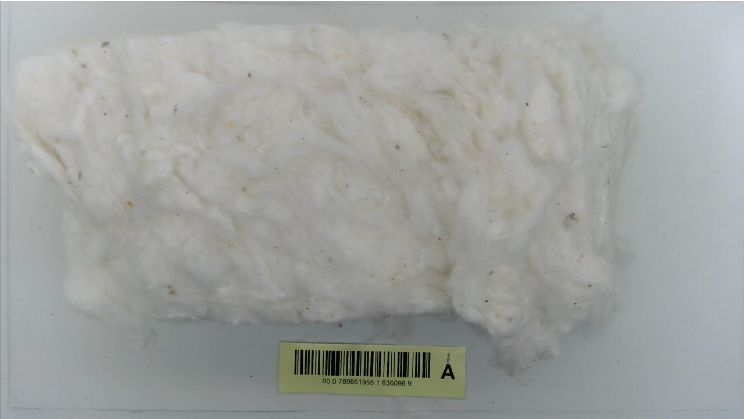
\includegraphics[width=\textwidth]{images/1_amostra_original.pdf}
            \caption{Imagem Bruta (Original)}
            \label{fig:pipe_a}
        \end{subfigure}
        \hfill
        \begin{subfigure}[b]{0.32\textwidth}
            \centering
            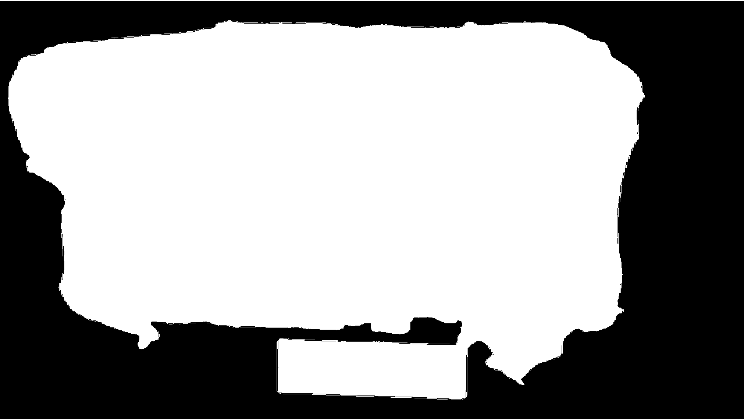
\includegraphics[width=\textwidth]{images/3_mascara_sem_fundo.pdf}
            \caption{Máscara BiRefNet}
            \label{fig:pipe_b}
        \end{subfigure}
        \hfill
        \begin{subfigure}[b]{0.32\textwidth}
            \centering
            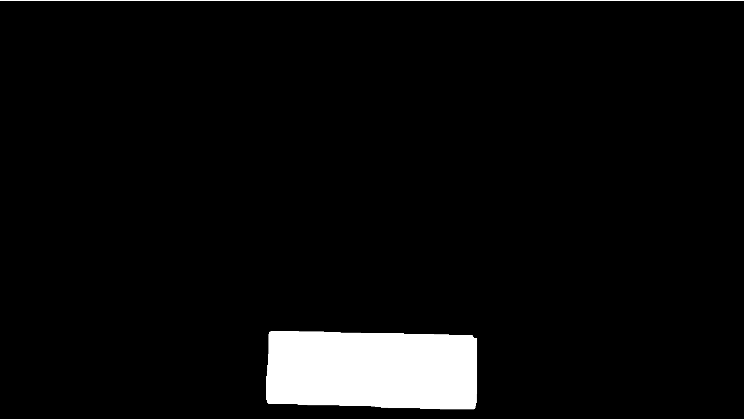
\includegraphics[width=\textwidth]{images/5_mascara_amarelo.pdf}
            \caption{Máscara da Etiqueta (HSV)}
            \label{fig:pipe_c}
        \end{subfigure}
        
        \vspace{0.4cm} % Espaço entre as linhas
        
        % Linha 2
        \begin{subfigure}[b]{0.32\textwidth}
            \centering
            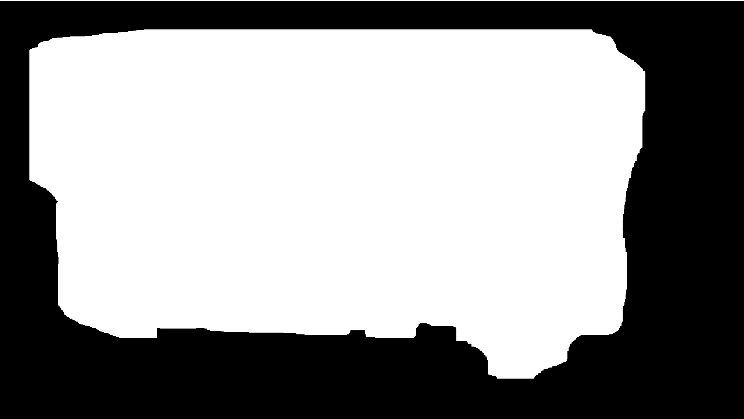
\includegraphics[width=\textwidth]{images/7_mascara_final.pdf}
            \caption{Máscara Final (Subtração)}
            \label{fig:pipe_d}
        \end{subfigure}
        \hfill
        \begin{subfigure}[b]{0.32\textwidth}
            \centering
            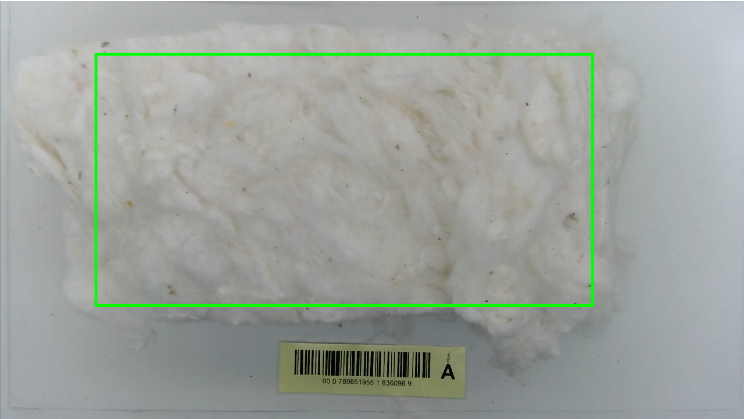
\includegraphics[width=\textwidth]{images/8_retangulo_final.pdf}
            \caption{Maior Retângulo Interno (LIR)}
            \label{fig:pipe_e}
        \end{subfigure}
        \hfill
        \begin{subfigure}[b]{0.32\textwidth}
            \centering
            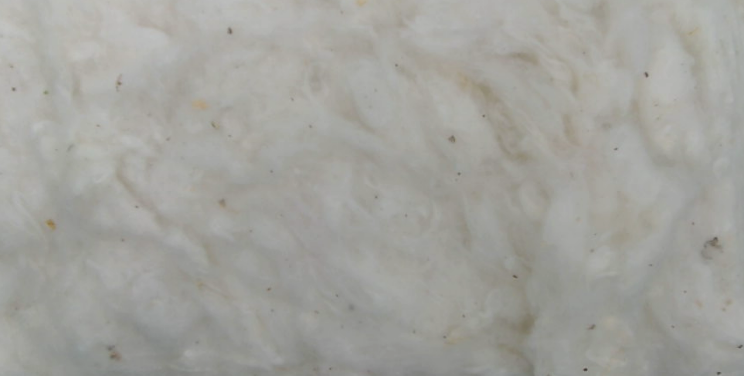
\includegraphics[width=\textwidth]{images/9_imagem_recortada.pdf}
            \caption{Recorte Final (AOI)}
            \label{fig:pipe_f}
        \end{subfigure}
        
        \caption{Etapas sequenciais do \textit{pipeline} de pré-processamento visual: segmentação semântica, operações morfológicas para exclusão de ruídos e definição geométrica da Região de Interesse (AOI).}
        \label{fig:pipeline_completo}
    \end{figure}

\subsection{Engenharia de Características e Expansão Espectral}

    Para avaliar se a injeção de atributos morfológicos pré-computados favorece o desempenho das redes frente ao aprendizado puramente \textit{end-to-end} sobre as matrizes RGB (\textit{Red, Green, Blue}) originais, implementou-se uma ramificação paralela no \textit{pipeline} de pré-processamento. O objetivo foi aplicar a engenharia de características (\textit{feature engineering}) para a extração em multiescala das microtexturas da pluma de algodão.

    A técnica empregada baseou-se em bancos de filtros de Gabor bidimensionais. Por consistirem em funções Gaussianas moduladas por ondas senoidais, esses filtros são matematicamente eficientes para destacar estrias longitudinais, nós de fibras e bordas de micro-impurezas sob diversas perspectivas.

    Para a expansão dos dados, projetou-se um banco contendo 12 \textit{kernels} distintos, gerados pela permutação ortogonal de três frequências espaciais ($f \in \{0,05; 0,10; 0,20\}$) e quatro orientações angulares ($\theta \in \{0^\circ, 45^\circ, 90^\circ, 135^\circ\}$), mantendo-se uma largura de banda (\textit{bandwidth}) constante e ajustada em 0,7. O canal de luminância de cada recorte (\textit{patch}) original foi convoluído com esses filtros. Em seguida, os 12 mapas de magnitude gerados foram empilhados em profundidade com os 3 canais RGB originais, transformando o dado em um tensor morfologicamente enriquecido de 15 canais. Esse conjunto de dados expandido foi salvo de forma isolada, servindo como matriz de entrada alternativa para os ensaios de viabilidade espectral.



\section{Construção do Conjunto de Dados, Rotulagem e Balanceamento de Classes}
\label{sec:conjunto_dados}

    %Revisado

O escopo desta dissertação foi direcionado às 10 classes comerciais de algodão em pluma mais prevalentes na produção local, em estrita conformidade com os padrões oficiais de classificação estabelecidos pela Instrução Normativa nº 24/2016 do Ministério da Agricultura, Pecuária e Abastecimento (MAPA). A rotulagem de cada amostra (\textit{ground truth}) foi estabelecida com base no laudo de classificação visual humano, adotado pela própria unidade de beneficiamento parceira. Esse procedimento assegurou que os rótulos atribuídos aos tensores de imagem correspondessem aos parâmetros utilizados nas operações reais de comercialização, conferindo validade industrial ao problema de classificação.

Após a etapa de pré-processamento (Camada \textit{Gold}), o conjunto de dados final consolidou-se em 7.908 \textit{patches} de imagem. Para a condução rigorosa dos experimentos, realizou-se a divisão dos dados utilizando uma proporção de 80\% para treinamento/validação (6.326 amostras) e 20\% para teste retido isoladamente (1.582 amostras).

É necessário destacar que essa divisão foi realizada de forma estratificada por classe, utilizando uma semente aleatória fixa (\textit{random seed} = 42). A estratificação garantiu que a proporção original de cada classe fosse preservada em ambas as partições. A distribuição quantitativa exata dos dados particionados é detalhada na Tabela \ref{tab:distribuicao_classes}.

\begin{table}[ht!]
    \centering
    \begin{threeparttable}
    \caption{Distribuição de amostras (\textit{patches}) por classe e partição do conjunto de dados.}
    \label{tab:distribuicao_classes}
    \begin{tabular}{c c c c}
        \hline
        \textbf{Classe Comercial} & \textbf{Treino/Validação (80\%)} & \textbf{Teste (20\%)} & \textbf{Total} \\
        \hline
        \textbf{31.2} & 1.126 & 281 & 1.407 \\
        \textbf{31.3} & 975 & 244 & 1.219 \\
        \textbf{31.4} & 1.112 & 278 & 1.390 \\
        \textbf{32.3} & 858 & 215 & 1.073 \\
        \textbf{32.4} & 275 & 69 & 344 \\
        \textbf{33.3} & 1.034 & 259 & 1.293 \\
        \textbf{41.4} & 238 & 59 & 297 \\
        \textbf{41.5} & 234 & 58 & 292 \\
        \textbf{42.4} & 302 & 76 & 378 \\
        \textbf{44.4} & 172 & 43 & 215 \\
        \hline
        \textbf{Total Geral} & \textbf{6.326} & \textbf{1.582} & \textbf{7.908} \\
        \hline
    \end{tabular}
    \begin{tablenotes}
        \small 
        \item \textit{Nota:} Divisão estratificada realizada antes da aplicação de técnicas de \textit{Data Augmentation}. Fonte: Do autor.
    \end{tablenotes}
    \end{threeparttable}
\end{table}

A referida distribuição quantitativa reflete o desbalanceamento natural intrínseco à produção agrícola, caracterizado por uma forte prevalência de qualidades superiores (ex: a classe majoritária 31.2 possui 1.407 amostras, enquanto a minoritária 44.4 possui apenas 215).

Para lidar com essa assimetria sem adulterar a distribuição estatística real do domínio de aplicação, o que poderia gerar viés de amostragem, optou-se por não aplicar técnicas de superamostragem artificial no disco. Em vez disso, a preservação da capacidade preditiva das classes minoritárias será tratada diretamente na fase de treinamento e validação dos modelos, por meio da adoção de métricas de otimização globalmente robustas a classes desbalanceadas, detalhadas na seção subsequente.



\section{Seleção e Adaptação dos Modelos Base (Modelos Avaliados)}
\label{sec:modelos}

    %Revisado

Para determinar a arquitetura mais adequada ao desafio multiescala da classificação da pluma de algodão (que exige tanto a análise global da cor quanto a detecção local de micro-impurezas), estruturou-se um \textit{benchmark} abrangente. Em vez de focar em uma única topologia, a pesquisa avaliou um espectro de modelos representativos dos principais paradigmas da visão computacional.

As arquiteturas foram instanciadas por meio da biblioteca \textit{TorchVision} do PyTorch \cite{paszke2017automatic} e agrupadas em três categorias de avaliação experimental:

\begin{enumerate}
    \item \textbf{Modelos baseados em autoatenção (\textit{Vision Transformers}):} Avaliou-se o ViT (\textit{Vision Transformer}) em suas variantes ViT-B/16 e ViT-B/32, além do Swin Transformer hierárquico nas versões \textit{Tiny} (Swin-T) e \textit{Small} (Swin-S). A inclusão dessas redes visou testar a capacidade dos mecanismos de atenção global na captura da uniformidade estrutural da fibra.
    
    \item \textbf{CNNs Modernas:} Testou-se a família EfficientNet (variantes B0, B1 e B2) e a arquitetura ConvNeXt (variantes \textit{Tiny} e \textit{Small}). O objetivo foi avaliar o balanço ótimo entre precisão de extração de características de granulação fina (\textit{fine-grained}) e viabilidade computacional em cenários de inferência rápida.
    
    \item \textbf{CNNs Clássicas (\textit{Baselines}):} Foram incluídas arquiteturas que consagraram o paradigma do aprendizado profundo, englobando redes com roteamento residual (ResNet-18, ResNet-34 e ResNet-50), conectividade densa (DenseNet-121 e DenseNet-169), topologias multiescala (Inception-v3) e modelos estritamente sequenciais (VGG-16 e VGG-19, ambas em suas versões otimizadas com \textit{Batch Normalization}).
\end{enumerate}

\subsection{Estratégia de \textit{Transfer Learning} e Customização do Topo (\textit{Classification Head})}

    Devido à complexidade inerente de se treinar arquiteturas ultraprofundas (especialmente os \textit{Transformers}) a partir de uma inicialização aleatória, com um conjunto de 7.908 tensores, adotou-se a estratégia de \textit{transfer learning} (Transferência de Aprendizado). 
    
    Todas as arquiteturas base listadas foram inicializadas com pesos pré-treinados no conjunto de dados genérico \textit{ImageNet-1K} (pesos padrão \texttt{IMAGENET1K\_V1}). Essa inicialização permitiu que as redes aproveitassem os filtros convolucionais primários, responsáveis pela detecção de bordas, contrastes e texturas básicas, acelerando a convergência e mitigando o risco de sobreajuste. Apenas as camadas finais foram submetidas ao processo de descongelamento de pesos (\textit{unfreezing}), cuja profundidade exata foi definida dinamicamente pelo algoritmo de otimização Optuna \cite{akiba2019optuna} para cada rede, conforme documentado no Apêndice \ref{apendice:optuna_search_spaces}.

    Por fim, como as arquiteturas originais são projetadas para classificar 1.000 categorias genéricas, o componente de classificação original (\textit{Classification Head}) de cada rede foi removido. Em sua substituição, acoplou-se um novo bloco classificador, estritamente projetado para o escopo desta pesquisa. 
    
    A nova estrutura conectada à saída da arquitetura base consistiu em: uma camada de redução de dimensionalidade por média global (\textit{Global Average Pooling} - GAP); uma camada de \textit{Dropout} (com taxa estocástica também regulada pelo Optuna entre $0,0$ e $0,7$, dependendo da propensão da rede ao \textit{overfitting}); e uma camada densa e linear final configurada com exatamente 10 neurônios de saída, correspondentes às 10 classes comerciais de qualidade da pluma de algodão avaliadas. A ativação preditiva final foi governada pela função \textit{Softmax} durante o cálculo da perda de entropia cruzada.

\section{Ambiente de treinamento e avaliação dos modelos}
\label{sec:ambiente_treinamento}

    %Revisado

Para garantir a reprodutibilidade e a execução sistemática dos experimentos, desenvolveu-se um ambiente automatizado de treinamento. A plataforma foi implementada na linguagem Python, utilizando o \textit{framework} PyTorch \cite{paszke2017automatic} devido à sua flexibilidade na manipulação de tensores e suporte nativo a grafos computacionais dinâmicos. O processamento foi acelerado em \textit{hardware} Apple Silicon (Mac M3), explorando o \textit{backend} MPS (\textit{Metal Performance Shaders}) para otimização da execução em GPU local. A gestão do ciclo de vida dos experimentos foi conduzida por meio da plataforma MLflow \cite{mlflow}, permitindo o rastreamento automatizado dos pesos das redes, hiperparâmetros testados e a evolução das métricas a cada época (\textit{epoch}), assegurando a transparência e rastreabilidade total do processo.

\subsection{Regularização e Aumento de Dados Dinâmico)}

    Como o conjunto de dados original foi particionado sem a aplicação de superamostragem estática, a mitigação do viés de classes e a prevenção de sobreajuste (\textit{overfitting}) foram tratadas de forma dinâmica durante o carregamento dos lotes (\textit{batches}). Para isso, implementou-se um \textit{pipeline} de aumento de dados estruturado em duas frentes complementares: transformações espaciais fotométricas intra-imagem e regularização avançada em nível de lote.

    A primeira frente foi orquestrada pela biblioteca Albumentations \cite{buslaev2020albumentations}. A cada época de treinamento, as imagens do conjunto de treino foram submetidas estocasticamente a rotações afins (até $45^\circ$), espelhamentos horizontais e verticais, além de variações de brilho e contraste. Essa abordagem garante a invariância rotacional do modelo, forçando-o a reconhecer a textura da pluma independentemente da sua orientação física na esteira de classificação. A segunda frente introduziu técnicas avançadas de regularização, especificamente o MixUp \cite{zhang2018mixup} e o CutMix \cite{yun2019cutmix}. Ao contrário do aumento tradicional, o MixUp realiza uma interpolação linear entre os \textit{pixels} e os rótulos de duas imagens aleatórias, enquanto o CutMix extrai um fragmento retangular de uma amostra e o sobrepõe em outra, mesclando as proporções de suas respectivas classes.

    A união dessas arquiteturas de aumento de dados com a técnica de suavização de rótulos (\textit{Label Smoothing}) \cite{szegedy2016rethinking} na função de perda de entropia cruzada (\textit{Cross-Entropy}) provou-se fundamental para o domínio agrícola estudado. Esse conjunto de restrições penaliza a formulação de predições superconfiantes e suaviza as fronteiras de decisão topológicas, incentivando as redes a focarem estritamente nas características morfológicas da pluma em vez de memorizarem ruídos esparsos ou artefatos de fundo.

\subsection{Otimização Bayesiana com Optuna}

    As arquiteturas modernas de \textit{deep learning} são altamente sensíveis à escolha de hiperparâmetros, cujo ajuste manual empírico é ineficiente e propenso a subotimizações. Para solucionar isso, o ajuste fino foi conduzido por meio de Otimização Bayesiana \cite{shahriari2016taking} utilizando o \textit{framework} Optuna. Empregou-se o algoritmo TPE (\textit{Tree-structured Parzen Estimator}) \cite{bergstra2011algorithms}, que modela a probabilidade condicional das métricas de desempenho dado um conjunto de hiperparâmetros, concentrando a busca em regiões promissoras do espaço paramétrico.

    O espaço de busca foi customizado dinamicamente para cada família de arquiteturas, abrangendo restrições específicas para as peculiaridades de cada rede. O detalhamento completo dos hiperparâmetros testados para cada modelo, bem como os seus respectivos limites de busca, encontra-se sumarizado no Apêndice \ref{apendice:optuna_search_spaces}. As variáveis otimizadas incluíram:
    
    \begin{itemize}
        \item \textbf{Profundidade do Ajuste Fino:} O número de camadas descongeladas (\textit{unfreeze layers}) para retreinamento, variando de acordo com a profundidade da rede (ex: poucas camadas para \textit{Vision Transformers} para preservar a extração genérica, e camadas mais profundas para CNNs tradicionais).
        \item \textbf{Taxa de Aprendizado (\textit{Learning Rate}):} Procura em escala logarítmica (entre $10^{-5}$ e $10^{-2}$), acoplada a agendadores de decaimento (\textit{Schedulers}) como \textit{Cosine Annealing Warm Restarts} \cite{loshchilov2017sgdr} e \textit{ReduceLROnPlateau}.
        \item \textbf{Decaimento de Peso (\textit{Weight Decay}):} Ajuste da regularização L2 para controle de complexidade dos pesos.
        \item \textbf{Otimizadores:} Alternância adaptativa entre SGD (com \textit{momentum}) para redes como ResNet, e AdamW \cite{loshchilov2019decoupled}, mandatório para a convergência de \textit{Transformers} e \textit{ConvNeXt}.
    \end{itemize}

\subsection{Função Objetivo Robusta para Desbalanceamento}

    No contexto algorítmico do estimador TPE, a formulação matemática da função objetivo dita o comportamento de toda a busca computacional. Minimizar diretamente a função de perda (\textit{loss}) ou maximizar a acurácia global em um conjunto de dados de pluma de algodão desbalanceado enviesaria o otimizador em favor dos hiperparâmetros que apenas classificam corretamente as classes majoritárias (como o Tipo 31.2). Para contornar essa subotimização latente, adotou-se a técnica de escalarização multiobjetivo \cite{knowles2006parego, paria2020escalarizacao}, estruturando-se uma função objetivo composta que funde a correlação estatística interclasses com a estabilidade geométrica do gradiente.

    A métrica base escolhida para ancorar a discriminação global da rede foi o Coeficiente de Correlação de Matthews (MCC) \cite{matthews1975comparison}, em virtude de sua robustez matemática inata perante o desequilíbrio de classes. O valor escalar $\mathcal{O}$, retornado ao Optuna para maximização ao final de cada iteração (\textit{trial}), foi calculado matematicamente pela expressão:

    $$ \mathcal{O} = \lambda_1 \left( \frac{\text{MCC} + 1}{2} \right) + \lambda_2 \left( e^{-\mathcal{L}_{val}} \right) $$

    em que a primeira parcela normaliza o MCC original (de $[-1, 1]$ para $[0, 1]$), ponderado pelo fator prioritário de classificação $\lambda_1 = 0,7$. A segunda parcela introduz um termo de qualidade baseado na perda de validação ($\mathcal{L}_{val}$), aplicando uma decadência exponencial ponderada por $\lambda_2 = 0,3$. Essa formulação garantiu que a busca Bayesiana priorizasse hiperparâmetros capazes de distinguir assertivamente todas as 10 classes de pluma, utilizando a suavidade da curva de perda apenas como critério de desempate técnico e estabilidade geométrica.


    % Para garantir a reprodutibilidade e a gestão sistemática dos experimentos, foi desenvolvido um ambiente automatizado de treinamento e avaliação. A plataforma foi implementada em Python, utilizando a biblioteca PyTorch como framework principal para a construção e o treinamento dos modelos de deep learning, devido à sua flexibilidade e vasto ecossistema.

    % A gestão do ciclo de vida dos experimentos foi realizada com a ferramenta MLflow. Esta plataforma permitiu o rastreamento automatizado de todos os artefatos experimentais, incluindo os hiperparâmetros utilizados, as métricas de performance (acurácia, perda), os modelos treinados e os gráficos de validação. Essa abordagem assegura a comparabilidade rigorosa entre os diferentes modelos e facilita a análise dos resultados, granatindo a transparência do processo.

    % Para mitigar o overfitting e aumentar a capacidade de generalização dos modelos, foram empregadas as técnicas de regularização CutMix e MixUp em tempo real durante o treinamento, que combinam pares de imagens e seus rótulos para criar amostras sintéticas, incentivando o modelo a aprender representações mais robustas e a fazer predições menos confiantes em regiões ambíguas.

    % A otimização de hiperparâmetros foi conduzida de forma sistemática utilizando a biblioteca Optuna, que implementa algoritmos de busca avançados. Especificamente, foi empregada a Otimização Bayesiana com o algoritmo TPE (Tree-structured Parzen Estimator), pois é computacionalmente mais eficiente do que métodos como \textit{grid search} ou \textit{random search} para explorar eficientemente o espaço de hiperparâmetros (como taxa de aprendizado, intensidade do dropout e parâmetros do otimizador) e convergir rapidamente para as configurações que maximizam a acurácia de validação, garantindo assim que cada modelo fosse avaliado em sua performance ótima.


\section{Desenho Experimental}
\label{sec:desenho_experimental}

    %Revisado

Para consolidar o rigor científico desta pesquisa e permitir uma avaliação objetiva das arquiteturas selecionadas, formalizou-se um desenho experimental focado em responder às lacunas identificadas na literatura, especificamente quanto ao \textit{trade-off} entre o poder de extração de características de granulação fina (\textit{fine-grained}) e a eficiência computacional.

\subsection{Fases da Experimentação e Questões de Pesquisa do Estudo}

    Em vez de concentrar a avaliação em um único teste estático, o desenho metodológico desta pesquisa foi estruturado como uma sequência lógica de experimentos. A experimentação foi conduzida em três fases progressivas, cada qual desenhada para responder a uma Questão de Pesquisa (QP), testada estatisticamente por meio de uma hipótese nula correspondente.

    \subsubsection{Fase 1: Benchmark Global}

        Esta fase consistiu na avaliação cruzada de todas as arquiteturas sob as exatas mesmas condições de treinamento e hiperparâmetros. Esta etapa exploratória foi desenhada para testar a seguinte prova estrutural:

        \begin{itemize}
            \item\textbf{$H_{0,1}$ (Hipótese Nula):} Não existe diferença estatisticamente significativa no poder de generalização entre as diferentes famílias de arquiteturas avaliadas.
            \item\textbf{QP1:} Existe uma variação estatisticamente significativa no desempenho preditivo entre as topologias.
        \end{itemize}

    \subsubsection{Fase 2: Impacto da Temperatura de Cor}

        Esta fase analisou isoladamente o impacto das condições físicas de captura. Consistiu em reavaliar o desempenho das redes variando estritamente a temperatura de cor da iluminação (luz quente, fria e mista), com o objetivo de testar a seguinte premissa:

        \begin{itemize}
            \item\textbf{$H_{0,2}$ (Hipótese Nula):} A alteração física da iluminação no momento da captura não produz variação estatisticamente significativa no desempenho preditivo dos modelos.
            \item\textbf{QP2:} A otimização espectral da iluminação exerce um impacto positivo e estatisticamente significativo no desempenho preditivo universal.
        \end{itemize}

    \subsubsection{Fase 3: Expansão Espectral}

        A última fase experimental avaliou a utilidade técnica da injeção de conhecimento morfológico explícito. Consistiu em expandir os tensores de entrada utilizando bancos de filtros de Gabor clássicos, com o intuito de validar a seguinte hipótese:

        \begin{itemize}
            \item\textbf{$H_{0,3}$ (Hipótese Nula):} A expansão espectral por meio de \textit{feature engineering} não altera de forma estatisticamente significativa a capacidade discriminativa dos classificadores em relação ao aprendizado sobre matrizes RGB puras.
            \item\textbf{QP3:} A injeção de características morfológicas pré-computadas eleva de forma estatisticamente significativa a precisão dos classificadores, mostrando-se mais eficiente do que o aprendizado \textit{end-to-end} estrito.
        \end{itemize}

    \subsubsection{Análise de Viabilidade Industrial}

        Complementarmente às três fases anteriores, avaliou-se ainda a seguinte questão:

        \begin{itemize}
            \item\textbf{QP4:} Qual arquitetura, dentre as avaliadas, oferece o melhor equilíbrio entre desempenho preditivo (MCC) e eficiência computacional (latência, FLOPs e \textit{footprint} de memória) para viabilizar a implantação em ambiente industrial de alta cadência?
        \end{itemize}

        Diferentemente de QP1--QP3, a QP4 não é testada por meio de uma hipótese nula formal, pois não se trata de uma comparação estatística binária entre dois grupos, mas de uma análise descritiva e comparativa de ranking multicritério (Seção \ref{sec:viabilidade_industrial}).


\subsection{Métricas de Avaliação}

    Devido ao inerente desbalanceamento de classes dos dados deste estuvo, a acurácia global foi monitorada apenas como métrica de referência estrutural, uma vez que ela pode apresentar um viés otimista ao mascarar o erro nas classes minoritárias. A avaliação definitiva da capacidade de generalização dos modelos baseou-se nas seguintes métricas:

    \begin{enumerate}
        \item \textbf{\textit{F1-Score} Macro:} Avalia a média harmônica entre a precisão (\textit{precision}) e a revocação (\textit{recall}). O cálculo \textit{macro} computa a métrica separadamente para cada uma das 10 classes comerciais e extrai a média aritmética não ponderada. Isso garante que as classes minoritárias (ex: Tipo 44.4) exerçam o mesmo peso na avaliação final que as majoritárias (ex: Tipo 31.2).
        
        \item \textbf{Coeficiente de Correlação de Matthews (MCC):} Considerada uma das métricas mais confiáveis para avaliação multiclasse em conjuntos de dados severamente desequilibrados. O MCC mede a correlação entre as predições e o \textit{ground truth}, retornando um valor no intervalo de $[-1, +1]$, no qual $+1$ representa uma predição perfeita, $0$ equivale a uma predição aleatória e $-1$ denota discordância total.
        
        \item \textbf{Coeficiente Kappa de Cohen ($\kappa$):} Estatística que mensura a concordância entre as predições do classificador e os rótulos reais, compensando a probabilidade de essa concordância ocorrer puramente ao acaso. É uma métrica crucial para o domínio agrícola, pois penaliza severamente modelos enviesados que adotam a estratégia de prever apenas a classe dominante.
        
        \item \textbf{Área Sob a Curva ROC (\textit{Receiver Operating Characteristic}), na média macro (\textit{macro ROC AUC}):} Mensura a capacidade discriminativa do modelo na separação das classes de qualidade, independentemente do limiar de decisão adotado pela função \textit{softmax}. Para o problema multiclasse, o cálculo foi realizado utilizando a abordagem Um-Contra-Todos (\textit{One-vs-Rest} - OvR) para cada tipo de algodão, extraindo-se em seguida a média não ponderada (\textit{macro}).
        
        \item \textbf{Matriz de Confusão:} Utilizada para a análise qualitativa detalhada dos erros interclasses. Permite diagnosticar se os modelos estão confundindo amostras de algodão vizinhas no espectro de qualidade (ex: classificar o Tipo 31.2 como 31.3 devido a variações sutis de amarelamento).
        
        \item \textbf{Eficiência Computacional:} Para chancelar a viabilidade da implementação da arquitetura vencedora em sistemas \textit{edge computing} na indústria, aferiu-se o número total de parâmetros treináveis (em milhões) e as Operações de Ponto Flutuante por Segundo (FLOPs), correlacionando esse custo com o ganho preditivo.
    \end{enumerate}

\subsection{Testes Estatísticos de Significância}

    A constatação empírica de que um modelo ``A'' obteve um MCC fracionariamente maior que um modelo ``B'' no conjunto de teste não é suficiente para decretar sua superioridade na literatura científica. Para garantir que as diferenças de desempenho observadas entre as melhores arquiteturas não decorreram de variações aleatórias da amostragem, aplicou-se o Teste Estatístico de McNemar.

    O Teste de McNemar é uma prova não paramétrica aplicada a tabelas de contingência $2 \times 2$, amplamente recomendada na literatura de aprendizado de máquina \cite{dietterich1998approximate} para comparar a proporção de erros e acertos de dois classificadores que foram avaliados sobre o exato mesmo conjunto de teste retido (\textit{holdout}). Adotou-se um nível de significância $\alpha = 0,05$ (Intervalo de Confiança de 95\%). Portanto, rejeitaram-se as respectivas Hipóteses Nulas ($H_{0,n}$) das fases experimentais apenas quando o valor-p (\textit{p-value}) resultante da comparação arquitetural foi inferior a $0,05$, atestando uma superioridade estatisticamente na classificação da pluma de algodão.
